% Copyright National ICT Australia 2005-2012
%	Author : Anthony Mak
%                Olivier Mehani
%		 William Uther
%
% This program can be redistributed and/or modified under the terms
% of the LaTeX Project Public License Distributed from CTAN
% archives in directory macros/latex/base/lppl.txt.

% If this template does not work, please check you have installed these.
% Required latex packages :-
%		Beamer class version 3.00 or higher
%		pgf version 0.63 or higher
%		xcolor version 2.00 or higher
%		(For details please read Beamer User Guide section 2.1 )
% Required NICTA Beamer Template files :-
%		(Make sure to include the following files in your TeX path)
%			beamerfontthemeNICTA.sty
%			beamercolorthemeNICTA.sty
%			beamercolorthemeNICTAsidebar.sty
%			beamerinnerthemeNICTA.sty
%			beamerouterthemeNICTA.sty
%			beamerthemeNICTA.sty

% /*** NO NEED TO MODIFY ***
\documentclass{beamer}
%\usetheme{NICTA}
%\usetheme[pagenum=false]{NICTA}
%\usetheme[sidebar=false, pagenum=false]{NICTA}
%\usetheme{Boadilla}
\usepackage{ANU-beamer}

% set the basic colors
%\definecolor{npurple} {RGB}{45,0,139}  % NICTA purple
%\definecolor{ngreen} {RGB}{65,170,0}  % NICTA green
%\definecolor{Gray}              {RGB}{139, 141, 142} 	% Gray  Approximate PANTONE COOL-GRAY-8
%\setbeamercolor{palette primary}   {fg=white,bg=ngreen!50}
%\setbeamercolor{palette secondary} {fg=white,bg=ngreen!60}
%\setbeamercolor{palette tertiary}  {fg=white,bg=ngreen!70}
%\setbeamercolor{palette quaternary}{fg=black,bg=white}
%\setbeamercolor{structure}{fg=ngreen!83}
%\setbeamercolor{titlelike}         {bg=Gray!10}
%\setbeamercolor{frametitle}        {bg=Gray!10}
%\setbeamercolor{cboxb}{fg=black,bg=ngreen!83}
%\setbeamercolor{cboxr}{fg=black,bg=red}
%
%% set colors for itemize/enumerate
%\setbeamercolor{item}{fg=ngreen!83}
%\setbeamercolor{item projected}{fg=white,bg=ngreen!83}
%
%% set colors for blocks
%\setbeamercolor{block title}{fg=ngreen!83,bg=white}
%\setbeamercolor{block body}{fg=black,bg=npurple!40}
%
%% set colors for alerted blocks (blocks with frame)
%\setbeamercolor{block alerted title}{fg=white,bg=ngreen!83}
%\setbeamercolor{block alerted body}{fg=black,bg=ngreen!10}
%
%% set the fonts
%\setbeamerfont{section in head/foot}{series=\bfseries}
%\setbeamerfont{block title}{series=\bfseries\sffamily}
%\setbeamerfont{block alerted title}{series=\bfseries}
%\setbeamerfont{frametitle}{series=\bfseries}
%\setbeamerfont{frametitle}{size=\Large}
%%\setbeamerfont{block body}{series=\rmfamily}
%%\setbeamerfont{caption}{series=\rmfamily\footnotesize}
%
%% set some beamer theme options
%\setbeamertemplate{title page}[default][colsep=-4bp,rounded=true]
%\setbeamertemplate{sections/subsections in toc}[square]
\setbeamertemplate{items}[circle]
%\setbeamertemplate{blocks}[width=0.0]
%\beamertemplatenavigationsymbolsempty

%\setbeamercolor*{palette secondary}{use=structure,fg=white,bg=red}
%\setbeamercolor*{palette tertiary}{use=structure,fg=white,bg=green}
%\usecolortheme{seahorse}

\usepackage[australian]{babel}
\usepackage{times}
\usepackage{xcolor}
\usepackage{booktabs,graphicx,multirow}
\usepackage[font={footnotesize}]{caption}
\captionsetup{compatibility=false}

% *** NO NEED TO MODIFY ***/
\usepackage[utf8]{inputenc}

%\usepackage{tikz}
%\usetikzlibrary{arrows, backgrounds, positioning, fit}


% *** Other stuff like notation ***/
%% Define bracket commands (normal, square and curly).
\newcommand{\brac} [1]  {\ensuremath{\left({#1}\right)}}
\newcommand{\sbrac}[1]  {\ensuremath{\left[{#1}\right]}}
\newcommand{\cbrac}[1]  {\ensuremath{\left\{{#1}\right\}}}
\newcommand{\abrac}[1]  {\ensuremath{\left\langle{#1}\right\rangle}}


%% Symbols

% General
\newcommand{\test}       {\ensuremath{^{*}}}
\newcommand{\testT}      {\ensuremath{^{*\top}\!}}
\newcommand{\ttest}      {\ensuremath{^{**}}}
\newcommand{\real}  [1] {\ensuremath{\mathbb{R}^{#1}}}
\newcommand{\ident} [1] {\ensuremath{\mathbf{I}_{#1}}}

% Variables
\newcommand{\lstate}    {\ensuremath{\mathbf{f}}}
\newcommand{\lcov}      {\ensuremath{\boldsymbol{\Sigma}}}
\newcommand{\obs}       {\ensuremath{\mathbf{y}}}
\newcommand{\hyper}     {\ensuremath{\boldsymbol{\theta}}}
\newcommand{\prmean}    {\ensuremath{\boldsymbol{\mu}}}
\newcommand{\prcov}     {\ensuremath{\mathbf{K}}}
\newcommand{\pomean}    {\ensuremath{\mathbf{m}}}
\newcommand{\pocov}     {\ensuremath{\mathbf{C}}}
\newcommand{\xcov}      {\ensuremath{\boldsymbol\Gamma_{\obs\pomean}}}
\newcommand{\Sobs}      {\ensuremath{\mathcal{Y}}}
\newcommand{\Sfunc}     {\ensuremath{\mathcal{M}}}
\newcommand{\scoef}     {\ensuremath{\kappa}}
\newcommand{\Sw}        {\ensuremath{w}}
\newcommand{\Kgain}     {\ensuremath{\mathbf{H}}}
\newcommand{\Linmat}    {\ensuremath{\mathbf{A}}}
\newcommand{\intcpt}    {\ensuremath{\mathbf{b}}}
\newcommand{\Fengy}     {\ensuremath{\mathcal{F}}}
\newcommand{\step}      {\ensuremath{\alpha}}
\newcommand{\jacob}[1]  {\ensuremath{\mathbf{J}_{#1}}}

% Augmented systems
\newcommand{\augobs}    {\ensuremath{\mathbf{z}}}
\newcommand{\augcov}    {\ensuremath{\mathbf{S}}}
\newcommand{\augLinmat} {\ensuremath{\mathbf{B}}}
\newcommand{\augintcpt} {\ensuremath{\mathbf{c}}}

% Gaussian Process
\newcommand{\obss}      {\ensuremath{y}}
\newcommand{\lstates}   {\ensuremath{f}}
\newcommand{\Lins}      {\ensuremath{a}}
\newcommand{\Linvec}    {\ensuremath{\mathbf{a}}}
\newcommand{\intcpts}   {\ensuremath{b}}
\newcommand{\inobs}     {\ensuremath{\mathbf{x}}}
\newcommand{\kernl}     {\ensuremath{k}}
\newcommand{\Kernl}     {\ensuremath{\mathbf{k}}}
\newcommand{\KERNL}     {\ensuremath{\mathbf{K}}}
\newcommand{\lvar}      {\ensuremath{\sigma^2}}
\newcommand{\lstd}      {\ensuremath{\sigma}}
\newcommand{\Lvar}      {\ensuremath{\boldsymbol\Lambda}}
\newcommand{\pomeans}   {\ensuremath{m}}
\newcommand{\pocovs}    {\ensuremath{C}}
\newcommand{\xcovs}     {\ensuremath{\Gamma}}
\newcommand{\khyper}    {\ensuremath{\theta}}
\newcommand{\khypers}   {\ensuremath{\boldsymbol\theta}}


%% Operations
\newcommand{\transpose}  {\ensuremath{^{\!\top}}}
\newcommand{\inv}        {\ensuremath{^{\text{-}1}}}
\newcommand{\deter}[1]   {\ensuremath{\left|{#1}\right|}}
\newcommand{\trace}[1]   {\ensuremath{\text{tr}\!\brac{#1}}}
\newcommand{\diag}[1]    {\ensuremath{\text{diag}\!\brac{#1}}}
\newcommand{\expec}[2]   {\ensuremath{\abrac{#2}_{\!{#1}}}}
\newcommand{\expece}[2]  {\ensuremath{\mathbb{E}_{#1}\!\sbrac{#2}}}
\newcommand{\evar} [2]   {\ensuremath{\mathbb{V}_{#1}\!\sbrac{#2}}}
\newcommand{\KL}[2]      {\ensuremath{\text{KL}\!\sbrac{{#1}\!\parallel\!{#2}}}}
\newcommand{\entropy}[1] {\ensuremath{\mathbb{H}\sbrac{#1}}}
\newcommand{\lnorm}[2]   {\ensuremath{\left\|{#2}\right\|_{{#1}}}}


%% Functions, PDFs etc
\newcommand{\nonlin}[1] {\ensuremath{g\!\brac{{#1}}}}
\newcommand{\augnonlin}[1] {\ensuremath{h\!\brac{{#1}}}}
\newcommand{\prob}  [1] {\ensuremath{p\!\brac{#1}}}
\newcommand{\probC} [2] {\ensuremath{p\!\left({#1}\middle\vert{#2}\right)}}
\newcommand{\qrob}  [1] {\ensuremath{q\!\brac{#1}}}
\newcommand{\qrobC} [2] {\ensuremath{q\!\left({#1}\middle\vert{#2}\right)}}
\newcommand{\gaus}  [1] {\ensuremath{\mathcal{N}\!\brac{#1}}}
\newcommand{\gausC} [2] {\ensuremath{\mathcal{N}\!\left({#1}\middle\vert{#2}\right)}}
\newcommand{\bern}  [1] {\ensuremath{\textrm{Bern}\!\brac{#1}}}
\newcommand{\bernC} [2] {\ensuremath{\textrm{Bern}\!\left({#1}\middle\vert{#2}\right)}}
\newcommand{\kfunc} [2] {\ensuremath{\kernl\!\brac{{#1}, {#2}}}}
\newcommand{\expon} [2] {\ensuremath{{#1}\!\times\!10^{#2}}}


%% Operators
\DeclareMathOperator*{\argmax}{\operatorname*{argmax}}
\DeclareMathOperator*{\argmin}{\operatorname*{argmin}}


\newsavebox\MBox
\newcommand\Cline[2][red]{{\sbox\MBox{$#2$}%
  \rlap{\usebox\MBox}\color{#1}\rule[-1.6\dp\MBox]{\wd\MBox}{0.7pt}}}

\begin{document}


%%%%% TITLE SLIDE %%%%%

\title[Extended and Unscented GPs]{Extended and Unscented Gaussian Processes}
\author[D. Steinberg \& E. Bonilla]{\textit{Daniel M.\ Steinberg} and
        Edwin V.\ Bonilla}

\institute[NICTA \& UNSW]{NICTA and The University of New South Wales} % Institution(s)
\date{}

\titlegraphic{
\includegraphics[width=2cm]{fig/logo-nicta}\hspace*{2cm}~%
   
\includegraphics[width=2cm]{fig/logo-unsw}
}

\begin{frame}
    \titlepage
\end{frame}


%%%%% FIRST SLIDE %%%%%

\begin{frame}
    \frametitle{Inverse Problems}

Many problems in science and engineering have some \textbf{forward} 
model, $\nonlin{\cdot}$, which is often nonlinear:
\begin{equation*}
    \obs = \nonlin{\lstate} + \boldsymbol\epsilon
\end{equation*}
\vspace{-6mm}
\begin{columns}

\begin{column}{0.5\linewidth}
\footnotesize
%\vspace{-3mm}

\begin{itemize}
    \item We can measure the outputs of the system, $\obs$, but the inputs,
        $\lstate$, are \textbf{latent}.
    \item We wish to infer these inputs \textbf{without} access to the inverse
        model, $\nonlininv{\cdot}$.
    \item $\obs$ may be a continuous process or path (robot arm motion), 
        so $\lstate$ is a \textbf{Gaussian Process}.
    \item The posterior, $\probC{\lstate}{\obs}$, is the solution to our
        inverse problem.
\end{itemize}

\end{column}

\begin{column}{0.5\linewidth}

\begin{figure}
    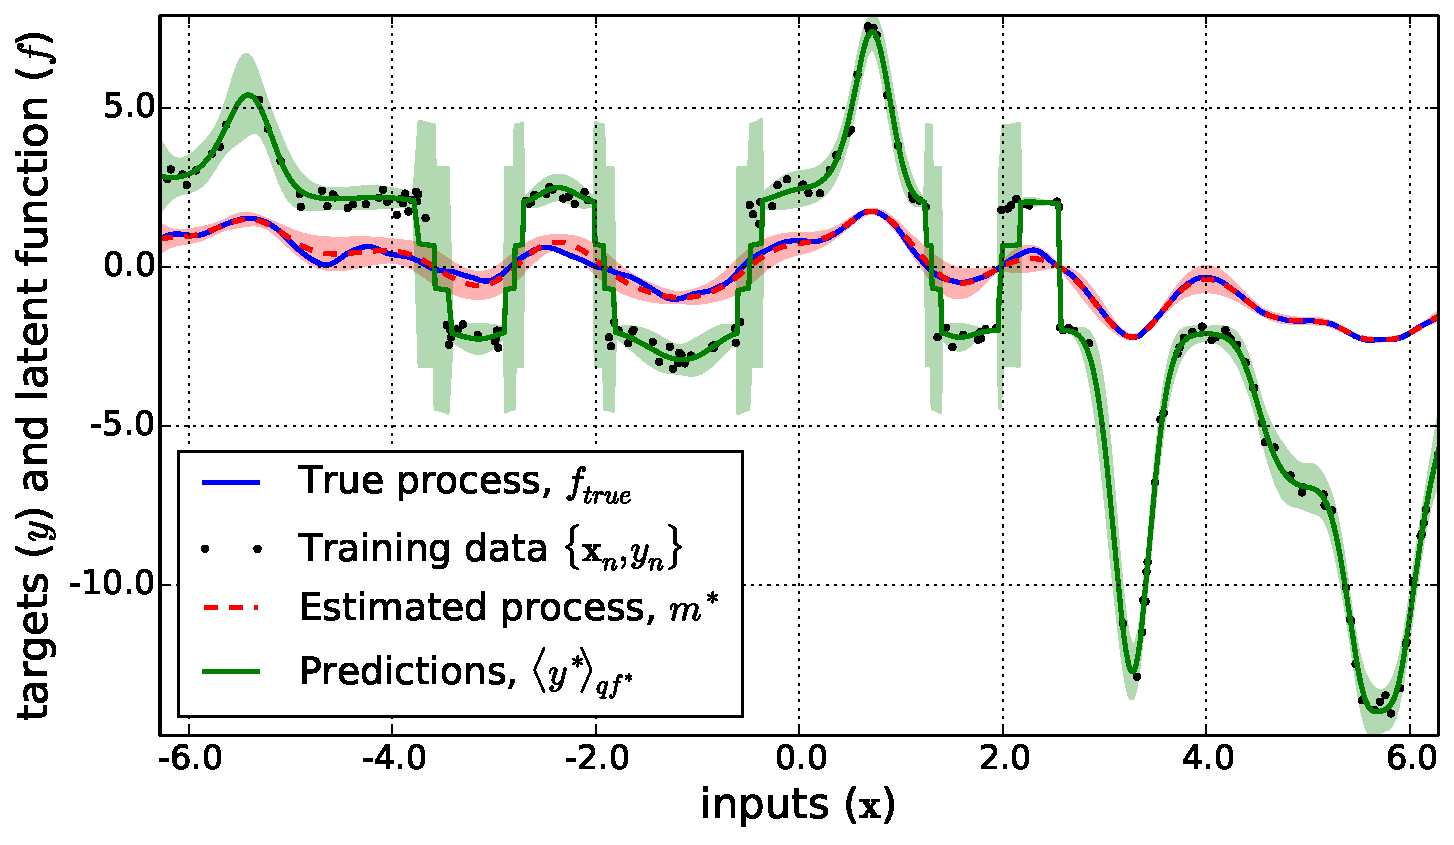
\includegraphics[width=0.75\linewidth]{fig/signdemo}

    \caption{Inferring a latent function, $\lstate$, from transformed and noisy
        realisations, $\obs$. Here $\nonlin{\lstate} =
        2\times\text{sign}\!\brac{\lstate} + \lstate^3$.}

    %\caption{The UGP with $\nonlin{\lstate} =
        %2\times\text{sign}\!\brac{\lstate} + \lstate^3$.}

\end{figure}

\end{column}
\end{columns}

\vspace{4mm}

\textbf{Problem}: Nonlinearities in the likelihood $\rightarrow$ 
\emph{intractable} posterior~$\probC{\lstate}{\obs}$.
\vspace{3mm}


\end{frame}


%%%%% SECOND SLIDE %%%%%

\begin{frame}
    \frametitle{Overview and Key Results}


\vspace{-4mm}
\begin{columns}

\begin{column}{0.45\linewidth}

Extended and unscented GPs,
\begin{itemize}
    \footnotesize
    \item Use \textbf{variational inference} to learn an approx.\ posterior 
        $\qrob{\lstate}$,
    \item with \textbf{Newton method} with linearization
        $\nonlin{\lstate} \approx \Linmat\lstate + \intcpt$;
    \begin{itemize}
        \footnotesize
        \item[EGP] 1\textsuperscript{st} order Taylor expansion
        \item[UGP] Unscented transform
    \end{itemize}
\end{itemize}

\vspace{5mm}
Some properties,
\begin{enumerate}
    \footnotesize
    \item No re-derivation needed for each new $\nonlin{\cdot}$,
    \item UGP does not require $\partial\nonlin{\lstate}\!/\partial{\lstate}$!
\end{enumerate}

\begin{block}{}
    \centering
    Poster -- \textbf{Wed33}
\end{block}

\end{column}

\begin{column}{0.55\linewidth}

\begin{figure}
    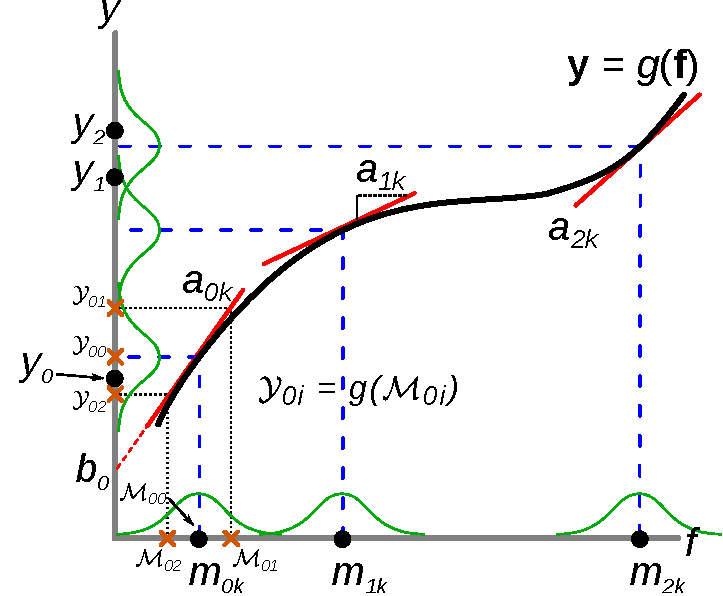
\includegraphics[width=0.65\linewidth]{fig/statlin_gp}

    \caption{UGP linearises $\nonlin{\cdot}$ using the unscented transform
        (regression).}

\end{figure}

\vspace{-1.1cm}

\begin{table}[tb]
    \centering
    \caption[]{Binary class.\ on USPS handwritten digits.}
    \tiny
    \vspace{-3mm}
    \begin{tabular}{r| c c}
    Algorithm & NLP $\obss\test$ & Error rate (\%) \\
    \toprule
    GP -- Laplace & 0.115& 2.975 \\
    GP -- EP & 0.075& 2.458 \\
    GP -- VB & 0.109 & 3.364 \\ 
    SVM (RBF) & 0.081 & 2.329 \\
    Logistic Reg. & 0.12 & 3.622 \\
    \midrule
    UGP & \emph{0.073} & \emph{1.941} \\
    EGP & 0.081 & 2.199 \\
    \bottomrule
    \end{tabular}
    \label{tab:class}
\end{table}

\end{column}


\end{columns}

\end{frame}

\end{document}
